\documentclass[11pt,a4paper,sans]{moderncv}

\moderncvstyle{casual}
\moderncvcolor{blue}

\usepackage{pdfpages}

\usepackage[scale=0.75]{geometry}
\setlength{\footskip}{54.40001pt}

\name{Alexander}{Starovoytov}
\email{stewk6@gmail.com}

\social[github]{stewkk}
\social[telegram]{stewkk}

\begin{document}

\makecvtitle{}

\section{Education}

\cventry{2017--2021}{High school}{Baumanskaya Engineering School №1580}{Moscow}{}{IT-class}
\cventry{2021--2025}{Undergraduate school}{BMSTU}{Moscow}{}{IU9, ``Department of Computer Science and Technologies''}

\section{Languages}

\cvlanguage{Russian}{}{native}
\cvlanguage{English}{B1-B2}{free reading of technical documentation}

\section{Hard skills}

\cvskillhead[-0.1em][Level][Skill][Years][Commentary]

\cvskillentry*{LG:}{4}{C}{1}{A one semester algorithms and data structures course in university.}
\cvskillentry{}{4}{C++}{4}{A wide experience of usage in olympiads. Also used in small projects. Learned both at school and at university. It's my main language.}
\cvskillentry{}{2}{Python}{3}{Learned at school. Periodically using it for small CP problems.}
\cvskillentry{}{3}{Bash}{2}{}
\cvskillentry{}{5}{Scheme (r5rs)}{1}{Introduction to functional programming course at university.}
\cvskillentry{}{3}{\LaTeX}{2}{Producing all of my doucuments in it.}
\cvskillentry{}{2}{Java}{1}{University OOP course.}
\cvskillentry{}{5}{Go}{1}{Main language at my university department. Also used it for my command project (Slavatidika).}
\cvskillentry{}{4}{Linux}{3}{The only operating system in my house. I enjoy linux server administration as much as tinkering my notebook setup.}
\cvskillentry{}{4}{Git}{3}{Using git on daily basis.}
\cvskillentry{}{4}{Docker}{2}{Building my projects in docker. It also used in deployment of all services at my home server.}

\section{Projects}

\cventry{2022}{Backend for
  Slavatidika}{\href{https://github.com/bmstu-iu9/ptp2022-8-todo-list}{Github}}{}{}{Canonical
  Go REST API with almost no external dependencies, docker
  production/development environment, CI/CD and Postgres as database.}

\section{Special education}
\cventry{2018--2019}{``Olympiad programming in C++''}{Baumanskaya Engineering School №1580}{}{}{Teacher: Partansky M.S.}
\cventry{2020--2021}{``Tinkoff Generation Algorithms and data structures''}{}{}{}{Level: B'}
\cventry{2010--2017}{Music school}{DMSH №3}{Sochi}{}{Piano}

\section{Achievements}
\cventry{2021}{№55. "Olympiad of school students «Step into the future»" (programming)}{}{winner}{}{}
\cventry{2020}{№55. "Olympiad of school students «Step into the future»" (programming)}{}{prizewinner}{}{}
\cventry{2020}{All-Russian Informatics Olympiad, regional stage}{}{Participant}{}{}
\cventry{2021}{All-Russian Informatics Olympiad, regional stage}{}{Participant}{}{}

\section{My free time}

In my spare time I usually enjoy:

\cvlistitem{tennis}
\cvlistitem{board games}
\cvlistitem{anime}

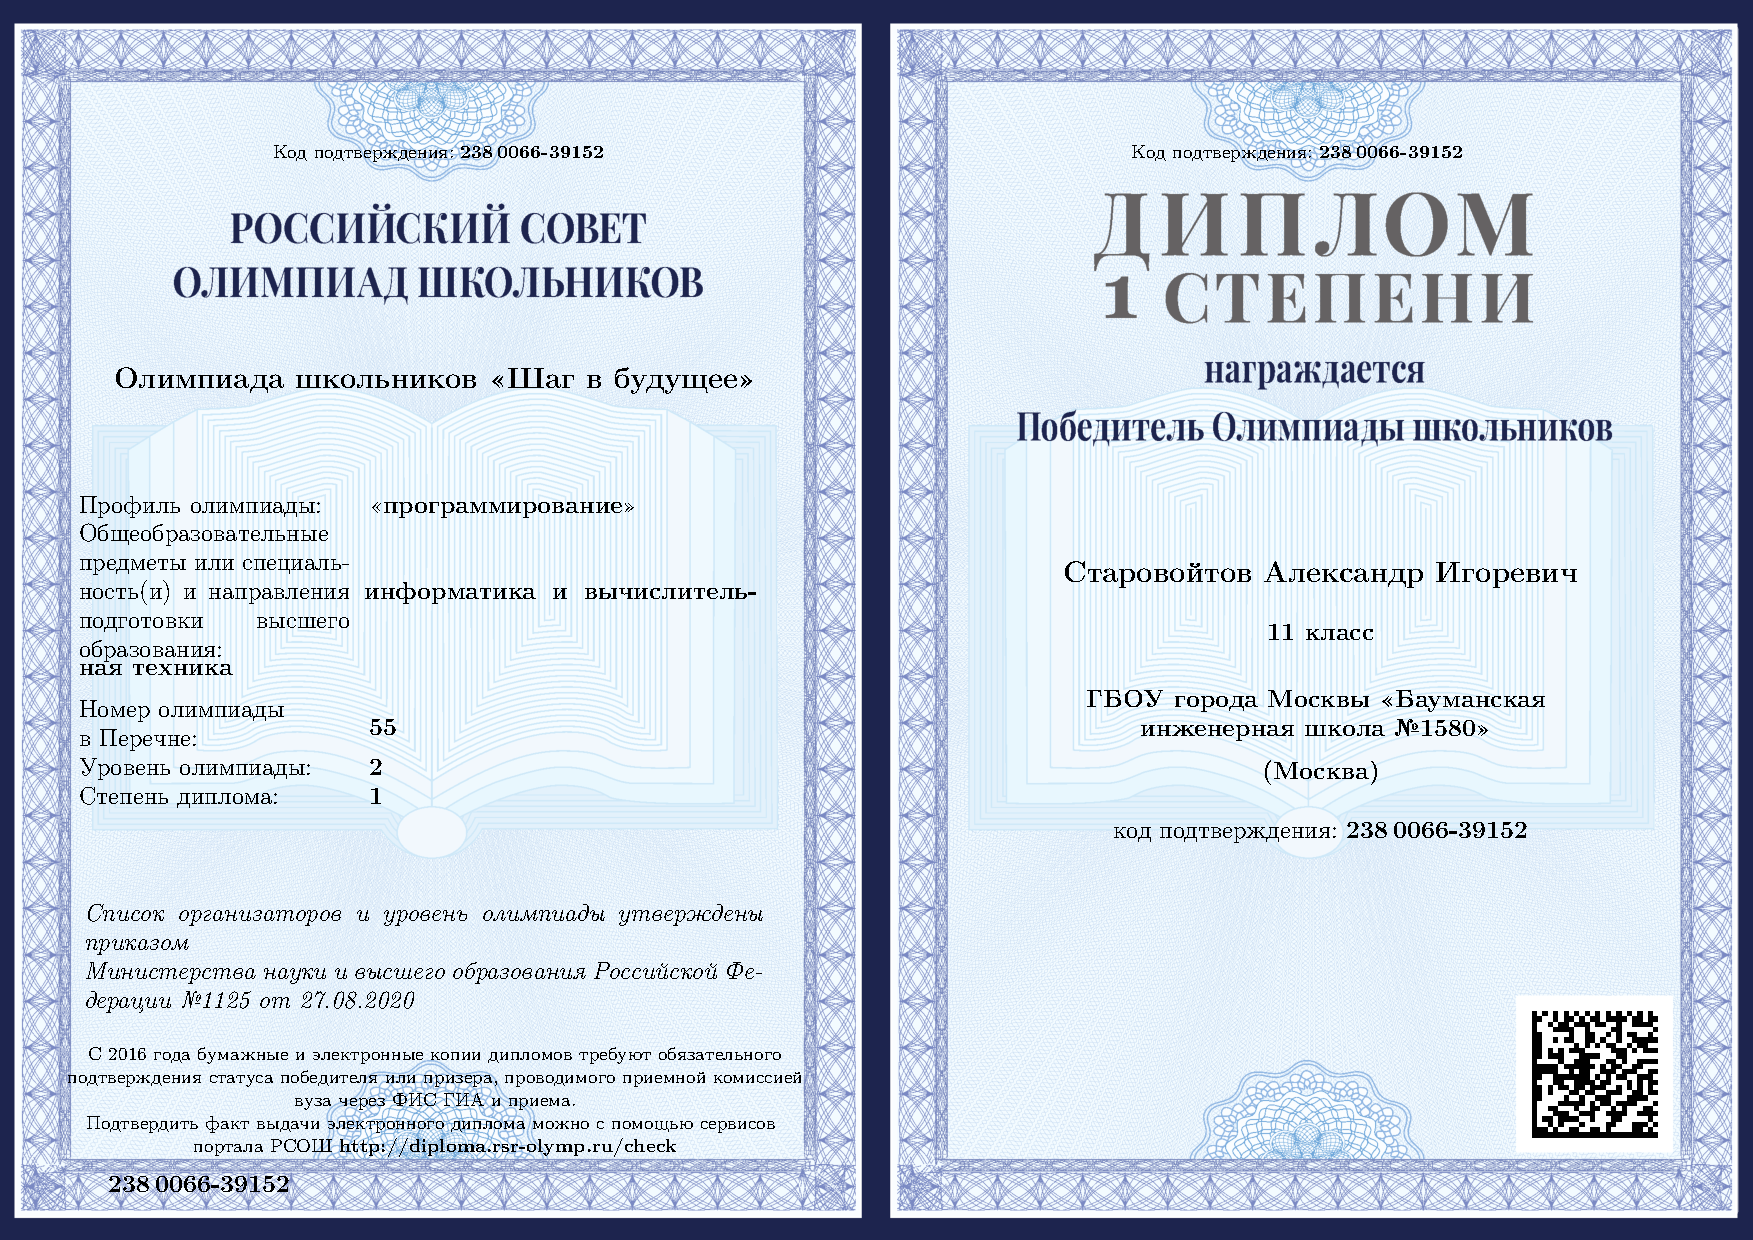
\includepdf[pages={1}]{color.pdf}
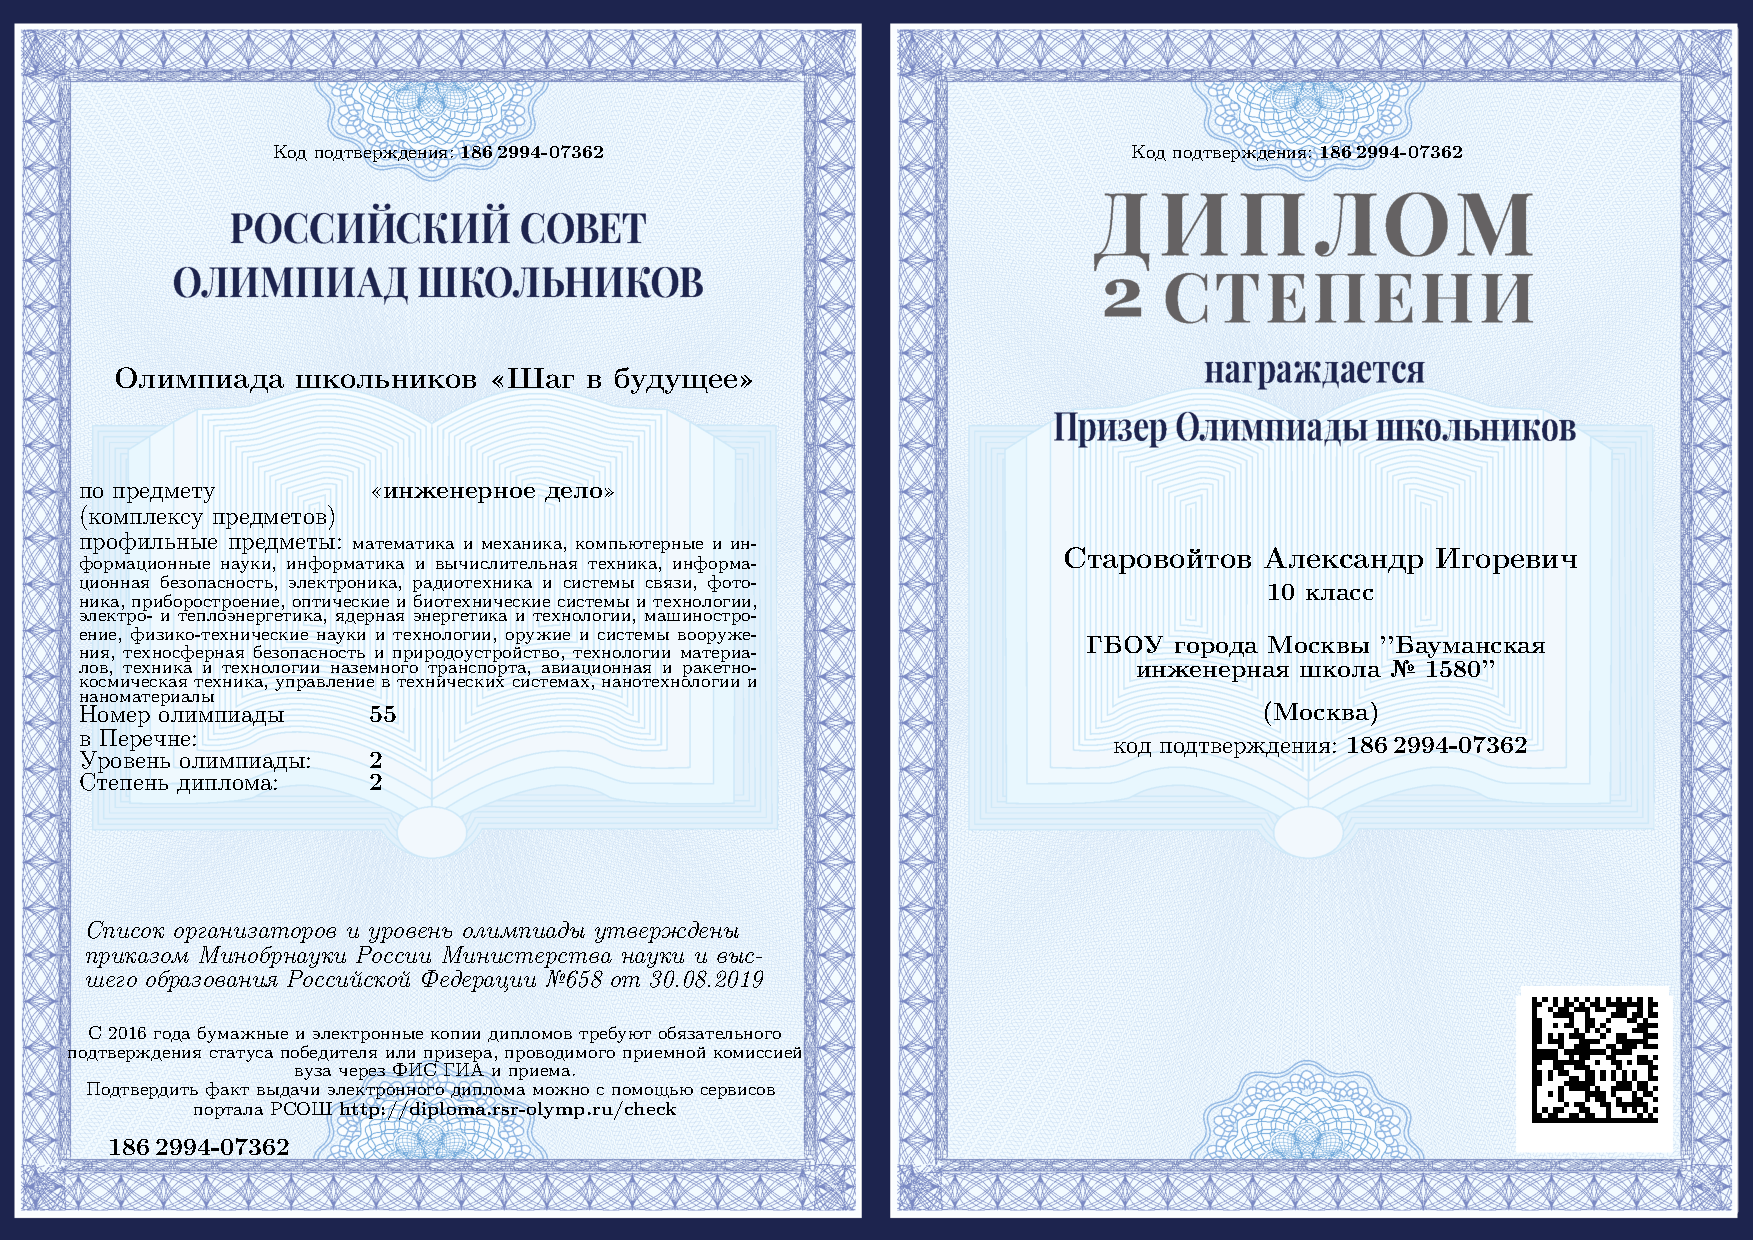
\includepdf[pages={1}]{color2.pdf}

\end{document}
